\begin{mainquestion}{ammeter}{Equivalent Circuits}
Consider the circuit shown below. An ammeter with an internal resistance of $R_{i}$ is used to measure the current flowing through a \qty{2}{\kilo\ohm} resistor between points $A$ and $B$.

\begin{center}
    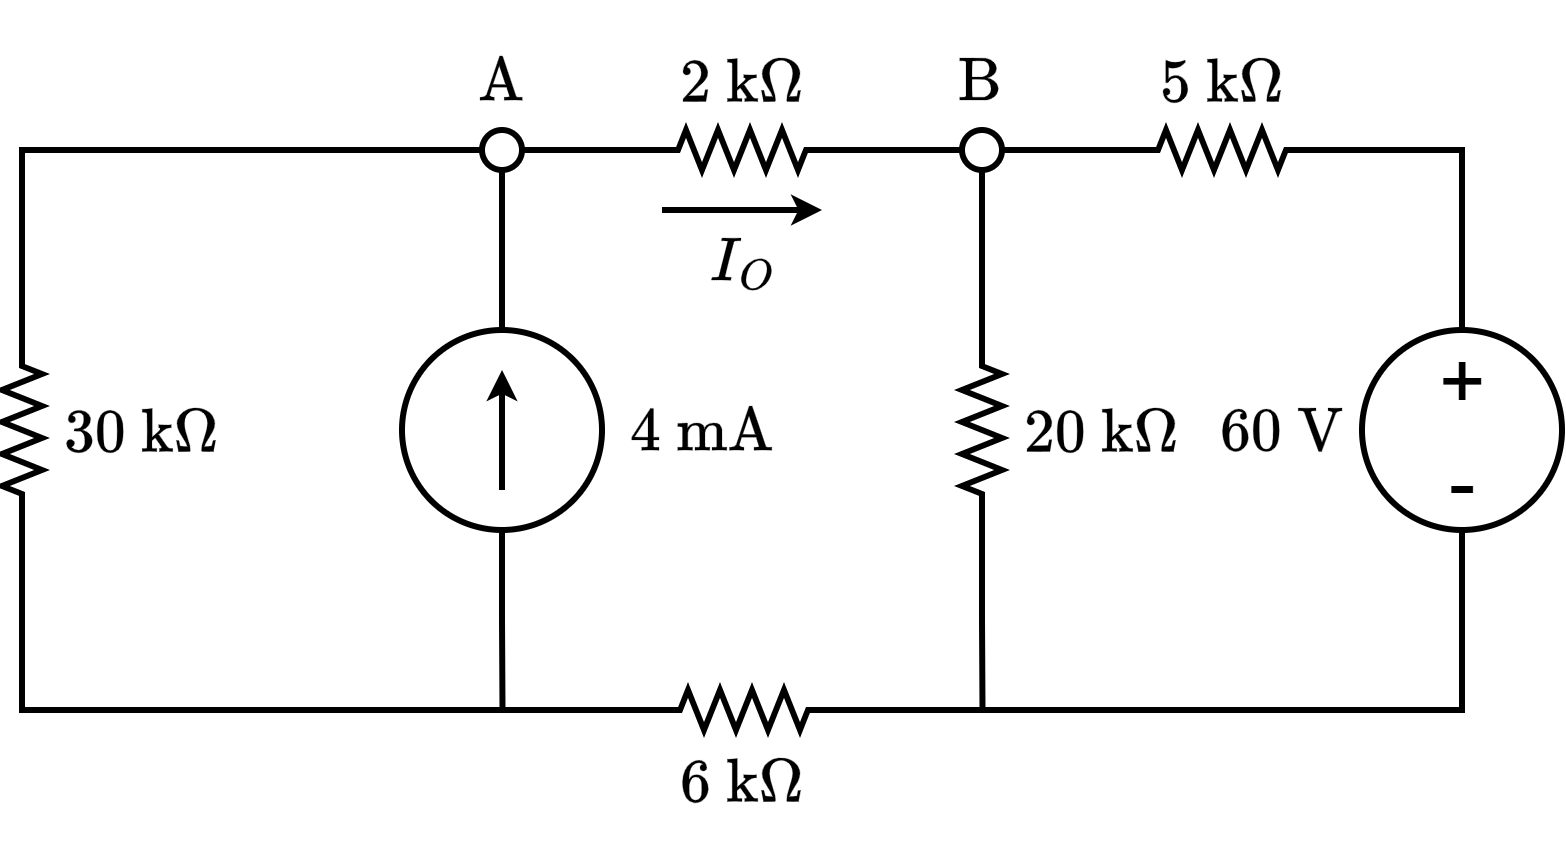
\includegraphics[width=5in]{circuit.png}
\end{center}

\begin{partquestion}{connection}{How should the ammeter be connected between $A$ and $B$? Show a sketch of the circuit (only include the portion between $A$ and $B$) which includes the ammeter with its internal resistance.}
\begin{answer}
The ammeter should be connected in series with the \qty{2}{\kilo\ohm} resistor between terminals $A$ and $B$. This means the current through the load passes through the ammeter and its internal resistance.

\begin{center}
    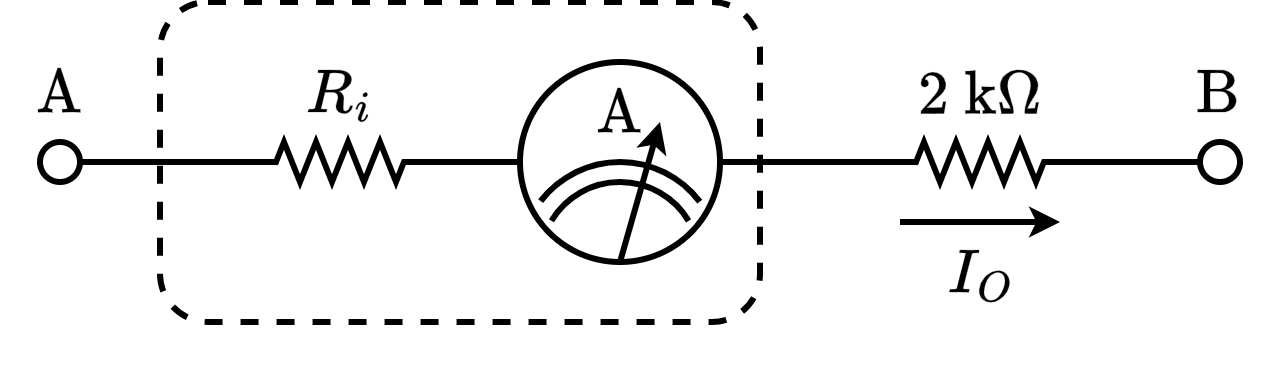
\includegraphics[width=0.7\textwidth]{ammeter_conn.png}
\end{center}
\end{answer}
\end{partquestion}

\begin{partquestion}{thevenin}{Find the Thévenin equivalent circuit at terminals $A$ and $B$ (without the \qty{2}{\kilo\ohm} load).}
\begin{answer}
To find the Thévenin resistance, we zero out all independent sources. The current source becomes an open circuit and the voltage source becomes a short circuit:

\begin{center}
    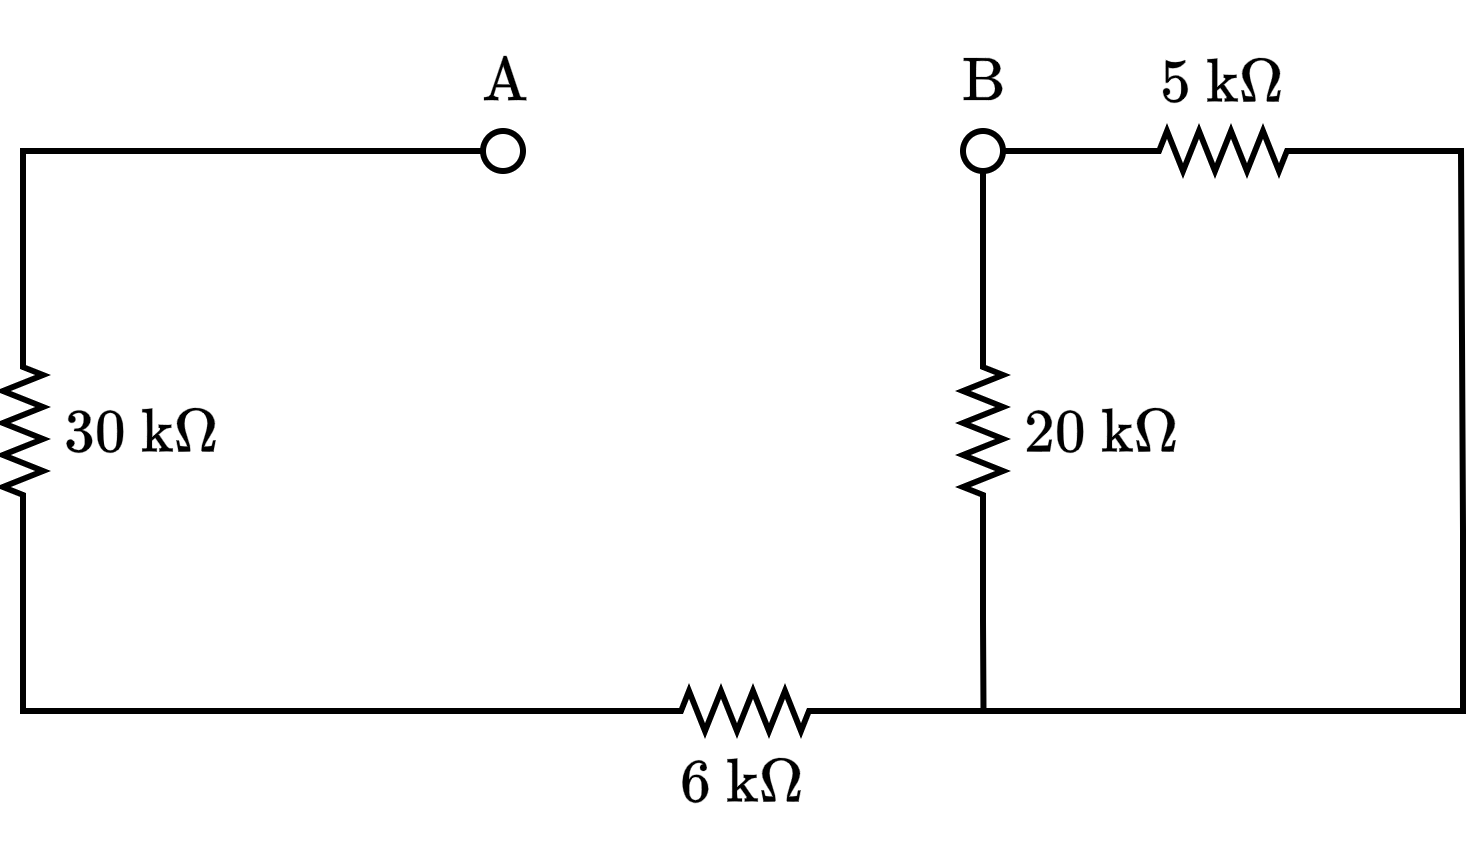
\includegraphics[width=0.7\textwidth]{rthev.png}
\end{center}

We can now combine the remaining resistors to find a single equivalent resistance.

\begin{align*}
    R_{TH} &= \qty{30}{\kilo\ohm} + \qty{6}{\kilo\ohm} + \qty{20}{\kilo\ohm}||\qty{5}{\kilo\ohm} \\
    &= \qty{36}{\kilo\ohm} + \frac{20\cdot5}{20+5}\unit{\kilo\ohm} \\
    &= \qty{40}{\kilo\ohm} \\
\end{align*}

\begin{center}
    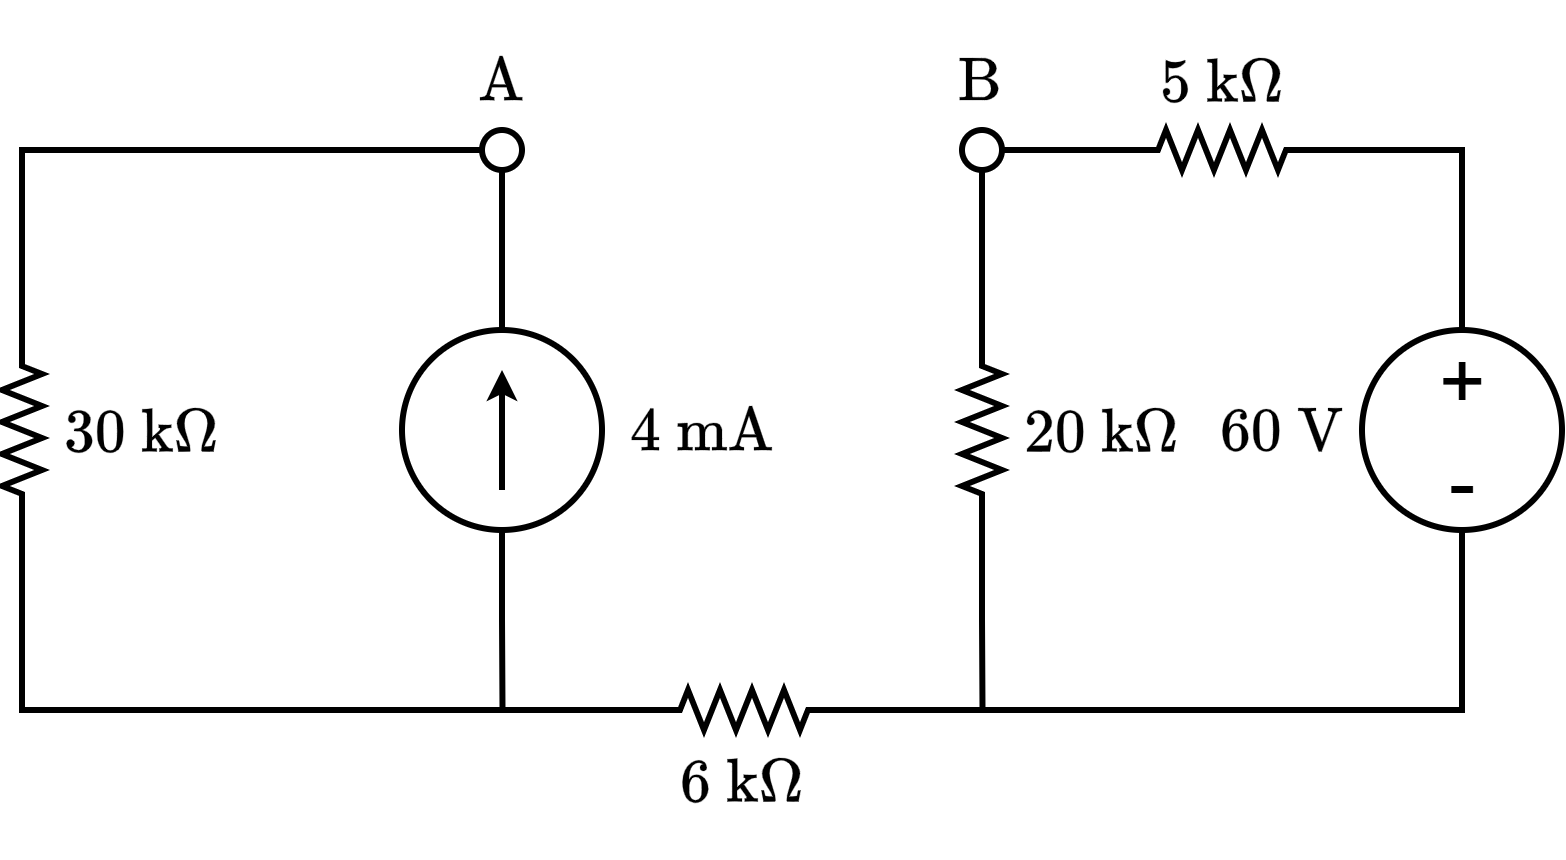
\includegraphics[width=4.5in]{thev_start.png}
\end{center}

Now to find the Thévenin voltage, compute the open-circuit voltage at $A$ and $B$. Because no current flows through the \qty{6}{\kilo\ohm} branch, its voltage is zero. The open-circuit voltage measured from $A$ to $B$ is therefore the voltage drop across the current source ($\qty{4}{\milli\ampere} \cdot\qty{30}{\kilo\ohm} = \qty{120}{\volt}$) minus the output of the voltage divider formed from the \qty{20}{\kilo\ohm} and \qty{5}{\kilo\ohm} resistors with the 60 V source ($60 \frac{20}{20 +5} = \qty{48}{\volt}$). Thus $V_{\text{TH}} = 120 - 48 = \qty{72}{\volt}$.

Now that we have both the Thévenin voltage and Thévenin resistance, we can combine them to find our equivalent circuit:

\begin{center}
    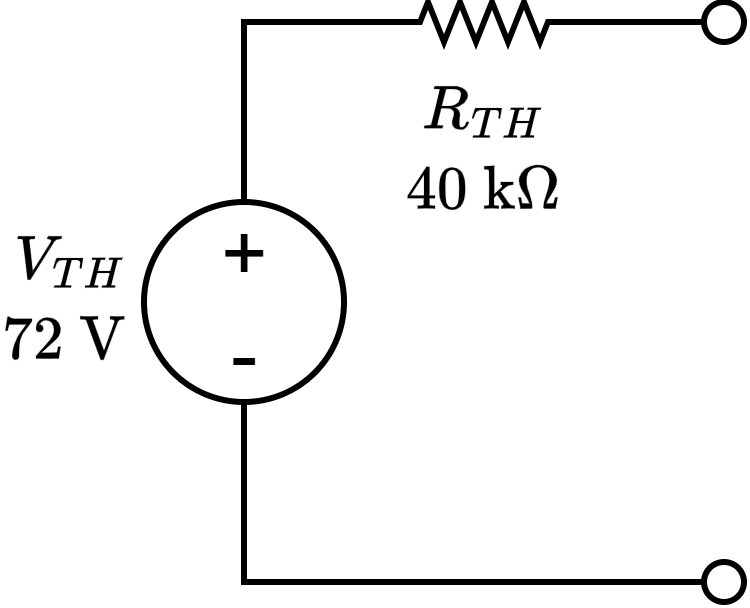
\includegraphics[width=2in]{thev_eq.png}
\end{center}
\end{answer}
\end{partquestion}

\begin{partquestion}{norton}{Find the Norton equivalent circuit at terminals $A$ and $B$ (without the \qty{2}{\kilo\ohm} load).}
\begin{answer}
Using the previously computed Thévenin equivalent, the Norton current is $I_{N} = V_{\text{TH}} / R_{\text{TH}} = \qty{72}{\volt} / \qty{40}{\kilo\ohm} = \qty{1.8}{\milli\ampere}$, and $R_{N} = \qty{40}{\kilo\ohm}$.

\begin{center}
    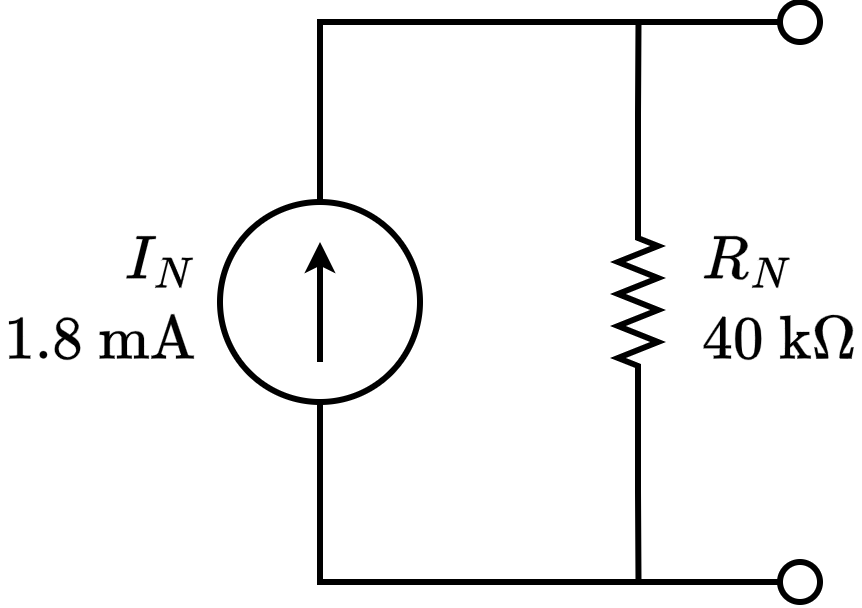
\includegraphics[width=2.2in]{norton_eq.png}
\end{center}
\end{answer}
\end{partquestion}

\begin{partquestion}{ri300}{What is the ammeter reading if $R_{i}=\qty{300}{\ohm}$?}
\begin{answer}
Using the Thévenin equivalent with $R_{i}=\qty{300}{\ohm}$ and $R_{L}=\qty{2}{\kilo\ohm}$ gives:
\[
I = \frac{V_{\text{th}}}{R_{\text{th}} + R_{i} + R_{L}} = \frac{72}{40{,}000 + 300 + 2000} \approx \qty{1.7}{\milli\ampere}.
\]
\end{answer}
\end{partquestion}

\begin{partquestion}{ri0}{What is the reading if $R_{i}=\qty{0}{\ohm}$?}
\begin{answer}
With $R_{i}=\qty{0}{\ohm}$ the current is:
\[
I = \frac{72}{40{,}000 + 0 + 2000} \approx \qty{1.71}{\milli\ampere}.
\]
Note that this is not a significant deviation, and in general will not be as long as the internal resistances are kept much lower than the loads through which we wish to measure current flow.
\end{answer}
\end{partquestion}

\end{mainquestion}
